\documentclass{beamer}
\usetheme{Boadilla}
\usepackage{essay-def}
\usepackage{bm}
\usepackage{amsfonts}
\usepackage{amssymb}
\usepackage{amsmath}
\usepackage{amsthm}
\usepackage{comment}
\usepackage{geometry}
\usepackage{hyperref}
\usepackage{subcaption}
\geometry{left=1cm,right=1cm}
    \title[Stability]{Sensitivity Analysis of Chaotic System}
\author[J. Zhao]{Jiaxi Zhao}
\date{9th October, 2023}
\begin{document}
\par \setlength{\parindent}{2em}

\begin{frame}
\titlepage

\end{frame}


\begin{frame}{Content}
	\begin{itemize}
		\item[$\bullet$] Chaotic Dynamics and Sensitivity Analysis
		\item[$\bullet$] {\color{red}Stability Analysis(TO DO)}
		\item[$\bullet$] Shadowing Lemma
		\item[$\bullet$] Least Square Shadowing (LSS)
		\item[$\bullet$] Numerical Experiments
	\end{itemize}
\end{frame}

\begin{frame}{Chaos}
	Chaos are ubiquitous in our life:
	\begin{itemize}
		\item[$\bullet$] Climate and weather forecasting
		\item[$\bullet$] Traffic flow
		\item[$\bullet$] Combustion and mixing
		\item[$\bullet$] Financial market
		\item[$\bullet$] Biological system
	\end{itemize}
	Lots of modern engineering problems are about modeling, quantifying, and controling 
	chaos.
\end{frame}

\begin{frame}{Sensitivity analysis of Chaos}
	Besides simulating the chaos, one of the most important task is sensitivity analysis of the
	chaos. This is especially important for controlling the chaos.
	\begin{itemize}
		\item[$\bullet$] Weather control: disaster mitigation, precipitation
		\item[$\bullet$] Fluid control: efficient mixing, combustion control
	\end{itemize}
	Moreover, sensitivity analysis is a key step to quantify and understand chaos.
\end{frame}

\begin{frame}{Lorenz dynamics}
	Consider the Lorenz system
	\begin{equation}\label{equ:Lorenz}
		\begin{aligned}
			\dot{x} & = \sigma(y - x),		\\
			\dot{y} & = \rho x - y - xz,		\\
			\dot{z} & = xy - \beta z,		\\
		\end{aligned}
	\end{equation}
	where $\sigma$ is the Prandtl number, $\rho$ Rayleigh number. Simple properties of the Lorenz Equations\footnotemark:
	\begin{itemize}
		\item[$\bullet$] \textbf{Nonlinearity}: coming from the nonlinear convection term.
		\item[$\bullet$] \textbf{Symmetry}: Equations are invariant under $(x, y) \rightarrow (-x, -y)$. Moreover,
the z-axis is invariant.
		\item[$\bullet$] \textbf{Fixed point}: $(0, 0, 0):$ stable fixed point for $0 < \rho < 1$, unstable otherwise;
		$(\sqrt{\beta(\rho-1)}, \sqrt{\beta(\rho-1)}, \rho-1), (-\sqrt{\beta(\rho-1)}, -\sqrt{\beta(\rho-1)}, \rho-1)$
		stable fixed points for $1<\rho<\frac{\sigma(\sigma+\beta+3)}{\sigma-\beta-1}\approx 24.74$.
	\end{itemize}
	\footnotetext{C. Sparrow, The Lorenz Equations: Bifurcations, Chaos, and Strange Attractors, Springer-Verlag, New York, 1982. }
\end{frame}

\begin{frame}{Lorenz dynamics}
	\begin{itemize}
		\item[$\bullet$] \textbf{Volume contraction}: The Lorenz system is dissipative
		\begin{equation}
			\frac{d}{dt}d\vol = \Tr(\nabla f)d\vol = -(\sigma + \beta + 1)d\vol.
		\end{equation}
		\item[$\bullet$] \textbf{Bounded attractor}: Consider the Lyapunov function 
		\begin{equation}
			V(x,y,z) = \rho x^2 + \sigma y^2 + \sigma(z-2\rho)^2.
		\end{equation}
		Together with the previous property guarantee the existence of a bounded globally attracting set 
		of measure $0$. This is the emergence of the strange attractor with fractal dimension.
	\end{itemize}
\end{frame}

\begin{frame}{Lorenz dynamics visualization}
	Lorenz dynamics has one of the key feature of the chaos: 

	\href{https://www.youtube.com/watch?v=FYE4JKAXSfY}{\textbf{Sensitive dependence on initial conditions:}}
	Given two trajectories, no matter how near they are at the initial condition, they will
	diverge exponentially fast until their distance reachs the size of the attractor basin. The deviation speed
	can be quantified by the first Lyapunov exponent.

	\begin{definition}[Formal definition]
		Chaos is aperiodic long-term behaviour in a deterministic system that 
	exhibits sensitive dependence on initial conditions.
	\end{definition}
\end{frame}

\begin{frame}{Quantifying chaotic dynamics: statistics}
	For chaotic dynamic, studying the trajectory-wise information is not a good choice
	due to the sensitive dependence on the inital condition. An alternative choice is to 
	use statistical quantities to describe the chaos, usually calculated along the trajectories
	\begin{equation}
		\la g \ra := \frac{1}{T}\sum_{k=1}^T g(\phi^k(\mfu)).
	\end{equation}
	
\end{frame}

\begin{frame}{Advantanges of statistics}
	\begin{itemize}
		\item[$\bullet$] 1. It is not sensitive to the initial condition via the Birkhoff's ergodic theorem:
		Let $\phi$ be an ergodic endomorphism of the probability space $X$ with invariant measure $\rho$ and let $g:X\rightarrow \mbR$ be a real-valued 
		measurable function. Then for almost $\forall \mfu \in X$, we have
		\begin{equation}
			\frac{1}{T}\sum_{k=1}^T g(\phi^k(\mfu)) = \int_X g(\mfu)d\rho(\mfu).
		\end{equation}
		\item[$\bullet$] 2. Statistics has important physical and engineering interpretation.
		\begin{itemize}
			\item[$\bullet$] Prediction weather $\Longleftrightarrow$ prediction climate
			\item[$\bullet$] Prediction pointwise fluid field $\Longleftrightarrow$ prediction the turbulence energy spectrum
			\item[$\bullet$] Prediction the pressure on the each area of a plane $\Longleftrightarrow$ predicting the average lifting 
			of the plane.
		\end{itemize} 
	\end{itemize}
\end{frame}

\begin{frame}{Next step: sensitivity analysis}
	Besides the value of the statistics $\la g \ra$, we are also interested in its dependence 
	over some parameters in order to understand the system better and control the system.

	Using Lorenz system as an example, we are interested in the following statistics
	\begin{equation}
		J(\rho) := \lim_{T\rightarrow \infty} \frac{1}{T}\int_0^T z_{\rho}(t)dt.
	\end{equation}
	Notice we involve $\rho$ Rayleigh number as a parameter of this statistics as we want to study
	the influence of $\rho$ on $J$. The other quantity of interest is the derivative $\frac{dJ}{d\rho}$ of $J$ over
	$\rho$.
\end{frame}

\begin{frame}{Sensitivity analysis: original method}
	Original method is given by linearizing the dynamics to obtain:
	\begin{equation}
		\frac{d}{dt}v(t) = \begin{pmatrix}
			-\sigma & \sigma & 0 \\
			\rho - z(t) & -1 & -x(t) 	 \\
			y(t) & x(t) & -\beta
		\end{pmatrix}v(t) + \begin{pmatrix}
			0 \\ x(t) \\ 0
		\end{pmatrix},
	\end{equation}
	{\color{red}This is method does not work for chaotic dynamics since the derivative operator (over $\rho$)
	and integration operator (over $t$) do not commute!!!}
	\begin{equation}
		\begin{aligned}
			& \ \frac{d}{d\rho}\lim_{T\rightarrow \infty} \frac{1}{T}\int_0^T z_{\rho}(t)dt 	\\
			\neq & \ \lim_{T\rightarrow \infty} \frac{1}{T}\int_0^T \frac{d}{d\rho}z_{\rho}(t)dt = \lim_{T\rightarrow \infty} \frac{1}{T}\int_0^T v_{z}(t)dt.
		\end{aligned}
	\end{equation}
\end{frame}

\begin{frame}{Pseudo-orbit}
	Given a map $f: X\rightarrow X$ of a metric space $(X, d)$ to itself, define a $\epsilon$-pseudo-orbit as a sequence of
$(\mfu_{n})$ of points such that $\mfu_{n+1}$ belongs to a $\epsilon$-neighborhood of $f(\mfu_n)$.
	\begin{example}[Parameterized family of dynamics]
		Consider a family of dynamical systems parameterized by $s$:
		\begin{equation}
			\mfu_{n+1} - f(\mfu_n, s).
		\end{equation}
		Given that $f$ is $L$-Lipschitz continuous w.r.t. $s$, any orbit of the dynamical system with 
		parameter $s+\delta s$ is a $L\delta s$-pseudo-orbit of the dynamical system with parameter $s$.
	\end{example}
\end{frame}

\begin{frame}{Pesudo-orbit}
	\begin{example}[Round-off error in numerical simulation]
		When numerically solving a dynamical system, due to the machine round-off error,
		in each step we are not performing the exact calculation but rather an $\epsilon$ approximation
		calculation assuming the state variable is bounded
		\begin{equation}
			\norml \mfu_{n+1} - f(\mfu_n) \normr < \epsilon f(\mfu_n).
		\end{equation}
	\end{example}
\end{frame}

\begin{frame}{Shadowing}
	\begin{theorem}[Shadowing lemma]
		Let $\Gamma$ be a hyperbolic invariant set of a diffeomorphism $f$. There exists a 
		neighborhood $U$ of $\Gamma$ with the following property: for any $\delta > 0$ there 
		exists $\epsilon > 0$, such that any (finite or infinite) $\epsilon$-pseudo-orbit that 
		stays in $U$ also stays in a $\delta$-neighborhood of some true orbit\footnotemark.
	\end{theorem}
	In a hyperbolic invariant set, the dynamics exhibit a combination of stable and unstable behavior.

	\href{https://www.youtube.com/watch?v=07jkQ1ox7vI&t=290s}{\textbf{Shadowing trajectory demo:}}
	\footnotetext{Pilyugin SY. Shadowing in dynamical systems. Lecture notes in mathematics, vol. 1706. Springer; 1999.}
\end{frame}

\begin{frame}{Digress: Stability in numerical linear algebra}
	\begin{itemize}
		\item[$\bullet$] A method for computing some result $w$ is forward stable if the computed solution $\wht w$
		is ``near'' the exact solution: 
		\begin{equation}
			\frac{\norml \wht w - w \normr_2}{\norml w \normr_2} < \epsilon.
		\end{equation}
		\item[$\bullet$] A method is backward stable if $\wht w$ is the exact solution of a perturbed problem; 
		that is, if $p$ is the problem satisfied by $w$ and $\wht p$ is the problem satisfied by $\wht w$, then 
		\begin{equation}
			\frac{\norml \wht p - p \normr_2}{\norml p \normr_2} < \epsilon.
		\end{equation}
	\end{itemize}
\end{frame}

\begin{frame}{Lesat square shadowing: Finding shadowing direction}
	Suppose we have a $s+\delta s$-trajectory:
	\begin{equation}
		\wht u^{t+1} = f(\wht u^t, s+\delta s), \quad u^t \in \mbR^n.
	\end{equation}
	Assume $f$ is uniform Lipschitz w.r.t. $s$, we know this is a $L\delta s$-pseudo orbit for the dynamics
	with parameter $s$. According to shadowing lemma, we could find $u^t$, s.t.
	\begin{equation}
		u^{t+1} = f(u^t, s), \quad u^t \in \mbR^n, \quad \norml \wht u^t - u^t \normr_2 < \epsilon, \ \forall t.
	\end{equation}
\end{frame}

\begin{frame}{Lesat square shadowing: vector version}
	To solve this, we formally write $\wht u^t = u^t + v^t \delta s$ and solve $v$ via optimization
	\begin{equation}\label{equ:vector-lss}
		\begin{aligned}
			& \min \sum_{t=1}^T \frac{\norml \wht u^t - u^t \normr_2^2}{\delta s^2} = \sum_{t=1}^T v_t^T v_t \\
			& s.t. \ v^{t+1} = \nabla_u f(u^t, s)v^t + \p_s f(u^t, s), \ t \in [T],
		\end{aligned}		
	\end{equation}
	where the constraint is nothing but the linearized dynamics. One can view this either as 
	a optimization over all the tangent vectors $v_t$ or simply over the initial condtion $v_1.$
\end{frame}

\begin{frame}{Solve LSS: Least square}
	Writing the linearized equation as a linear constraint
	\begin{equation}\label{equ:lss}
		\begin{aligned}
			& \min \sum_{t=1}^T v_t^T v_t \\
		&\begin{pmatrix}
			\mfI & -\nabla_u f(u_{T-1}) & \cdots & 0 & 0 \\
			0 & \mfI & \cdots & 0 & 0 \\
			0 & 0 & \cdots & 0 & 0 \\
			\vdots & \vdots & \ddots & \vdots & \vdots \\
			0 & 0 & \cdots & \mfI & -\nabla_u f(u_1)	\\
			0 & 0 & \cdots & 0 & 0
		\end{pmatrix}\begin{pmatrix}
			v_T \\ v_{T-1} \\ v_{T-2} \\ \vdots \\ v_2 \\ v_1
		\end{pmatrix} = \begin{pmatrix}
			\p_s f(u_{T-1}) \\ \p_s f(u_{T-2}) \\ \p_s f(u_{T-3}) \\ \vdots \\ \p_s f(u_{1}) \\ 0
		\end{pmatrix},
	\end{aligned}
	\end{equation}
	This is just a least square problem of size $T \times n$.
\end{frame}

\begin{frame}{Solve LSS: PMP}
	Even for moderate size system, e.g. simulating the 2D isotropic turbulence using Navier-Stokes equation with 
	grid size $32\times 32$ for $1000$ time step would result in a linear system of size 
	1e6 for each gradient evaluation, which is extremely expensive.
	
	Another method is viewing this as a control problem and solve it using PMP. In each gradient descent step,
	it requires to solve a forward primal problem followed by a backward adjoint problem. It become expensive 
	when forward problem solving is costable, e.g. LES.
\end{frame}

\begin{frame}{Sensitivity analysis of the Lorenz system}
	Going back to the Lorenz system, we consider the following statistics:
	\begin{equation}
		J(\rho) := \lim_{T\rightarrow \infty} \frac{1}{T}\int_0^T z_{\rho}(t)dt.
	\end{equation} 
	\begin{figure}[ht]
		\centering
			\centering
			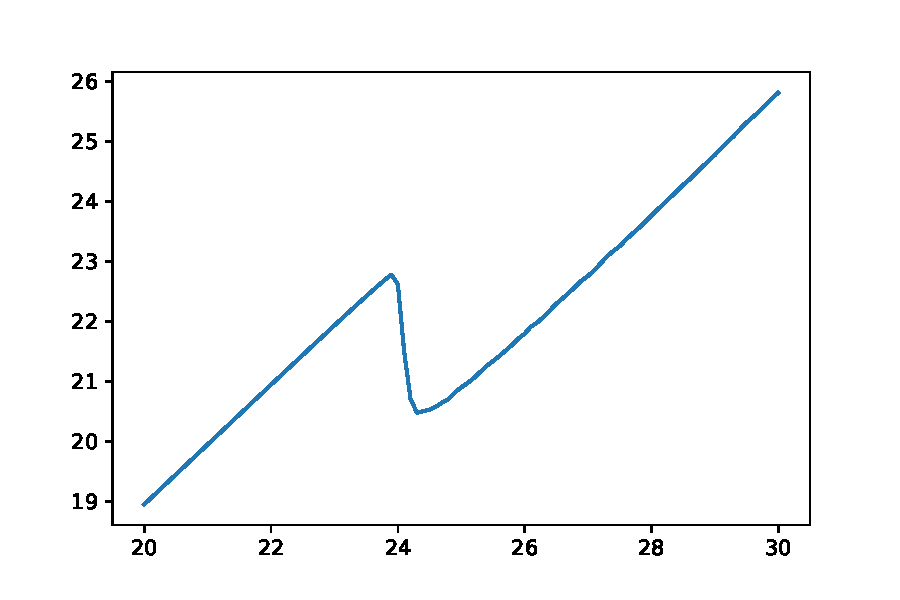
\includegraphics[width=.6\linewidth]{fig/rho-zbar.pdf}
			\caption{Dependence of the statistics $J(\rho)$ over parameter $\rho$. calculate
			using \textit{solve\_ivp} scipy routine with $T=100$ time unit and 100 random sample trajectories.}
	\end{figure}
\end{frame}

\begin{frame}{Sensitivity analysis of the Lorenz system}
	\begin{figure}[ht]
			\centering
			\begin{subfigure}{0.5\linewidth} % Adjust the width as needed
				\centering
				\includegraphics[width=\linewidth]{fig/Lorenz1.pdf}
				\caption{Gradient calcuated using naive method}
			  \end{subfigure}%
			  \begin{subfigure}{0.5\linewidth} % Adjust the width as needed
				\centering
				\includegraphics[width=\linewidth]{fig/Lorenz2.pdf}
				\caption{Gradient calcuated using LSS}
			  \end{subfigure}
			  \caption{Comparison of naive and LSS methods for sensitivity analysis}
	\end{figure}
\end{frame}

\begin{frame}{Subgrid modeling of the Kuramoto–Sivashinsky equation}
	Subgrid modeling is very important in the Large-eddy simulation. Here, we consider a simple 
	version of subgrid modeling for 1D KS equation:
	\bequ\label{KS}
	\p_t u + uu_x + u_{xx} + \nu u_{xxxx} = 0, \quad x \in [0, L],
	\eequ
	If we consider a coarse-grid model $\bar{u} = u * G$,
	\bequ
	\p_t \bar{u} +  \bar{u}\bar{u}_x +  \bar{u}_{xx} + (\nu+\Delta\nu)  \bar{u}_{xxxx} = 0, \quad x \in [0, L],
	\eequ
	Due to the nonlinearity, we need to add $\Delta \nu$. 
\end{frame}

\begin{frame}{Subgrid modeling of the Kuramoto–Sivashinsky equation}
	\begin{figure}[ht]
		\centering
		\begin{subfigure}{0.5\linewidth} % Adjust the width as needed
			\centering
			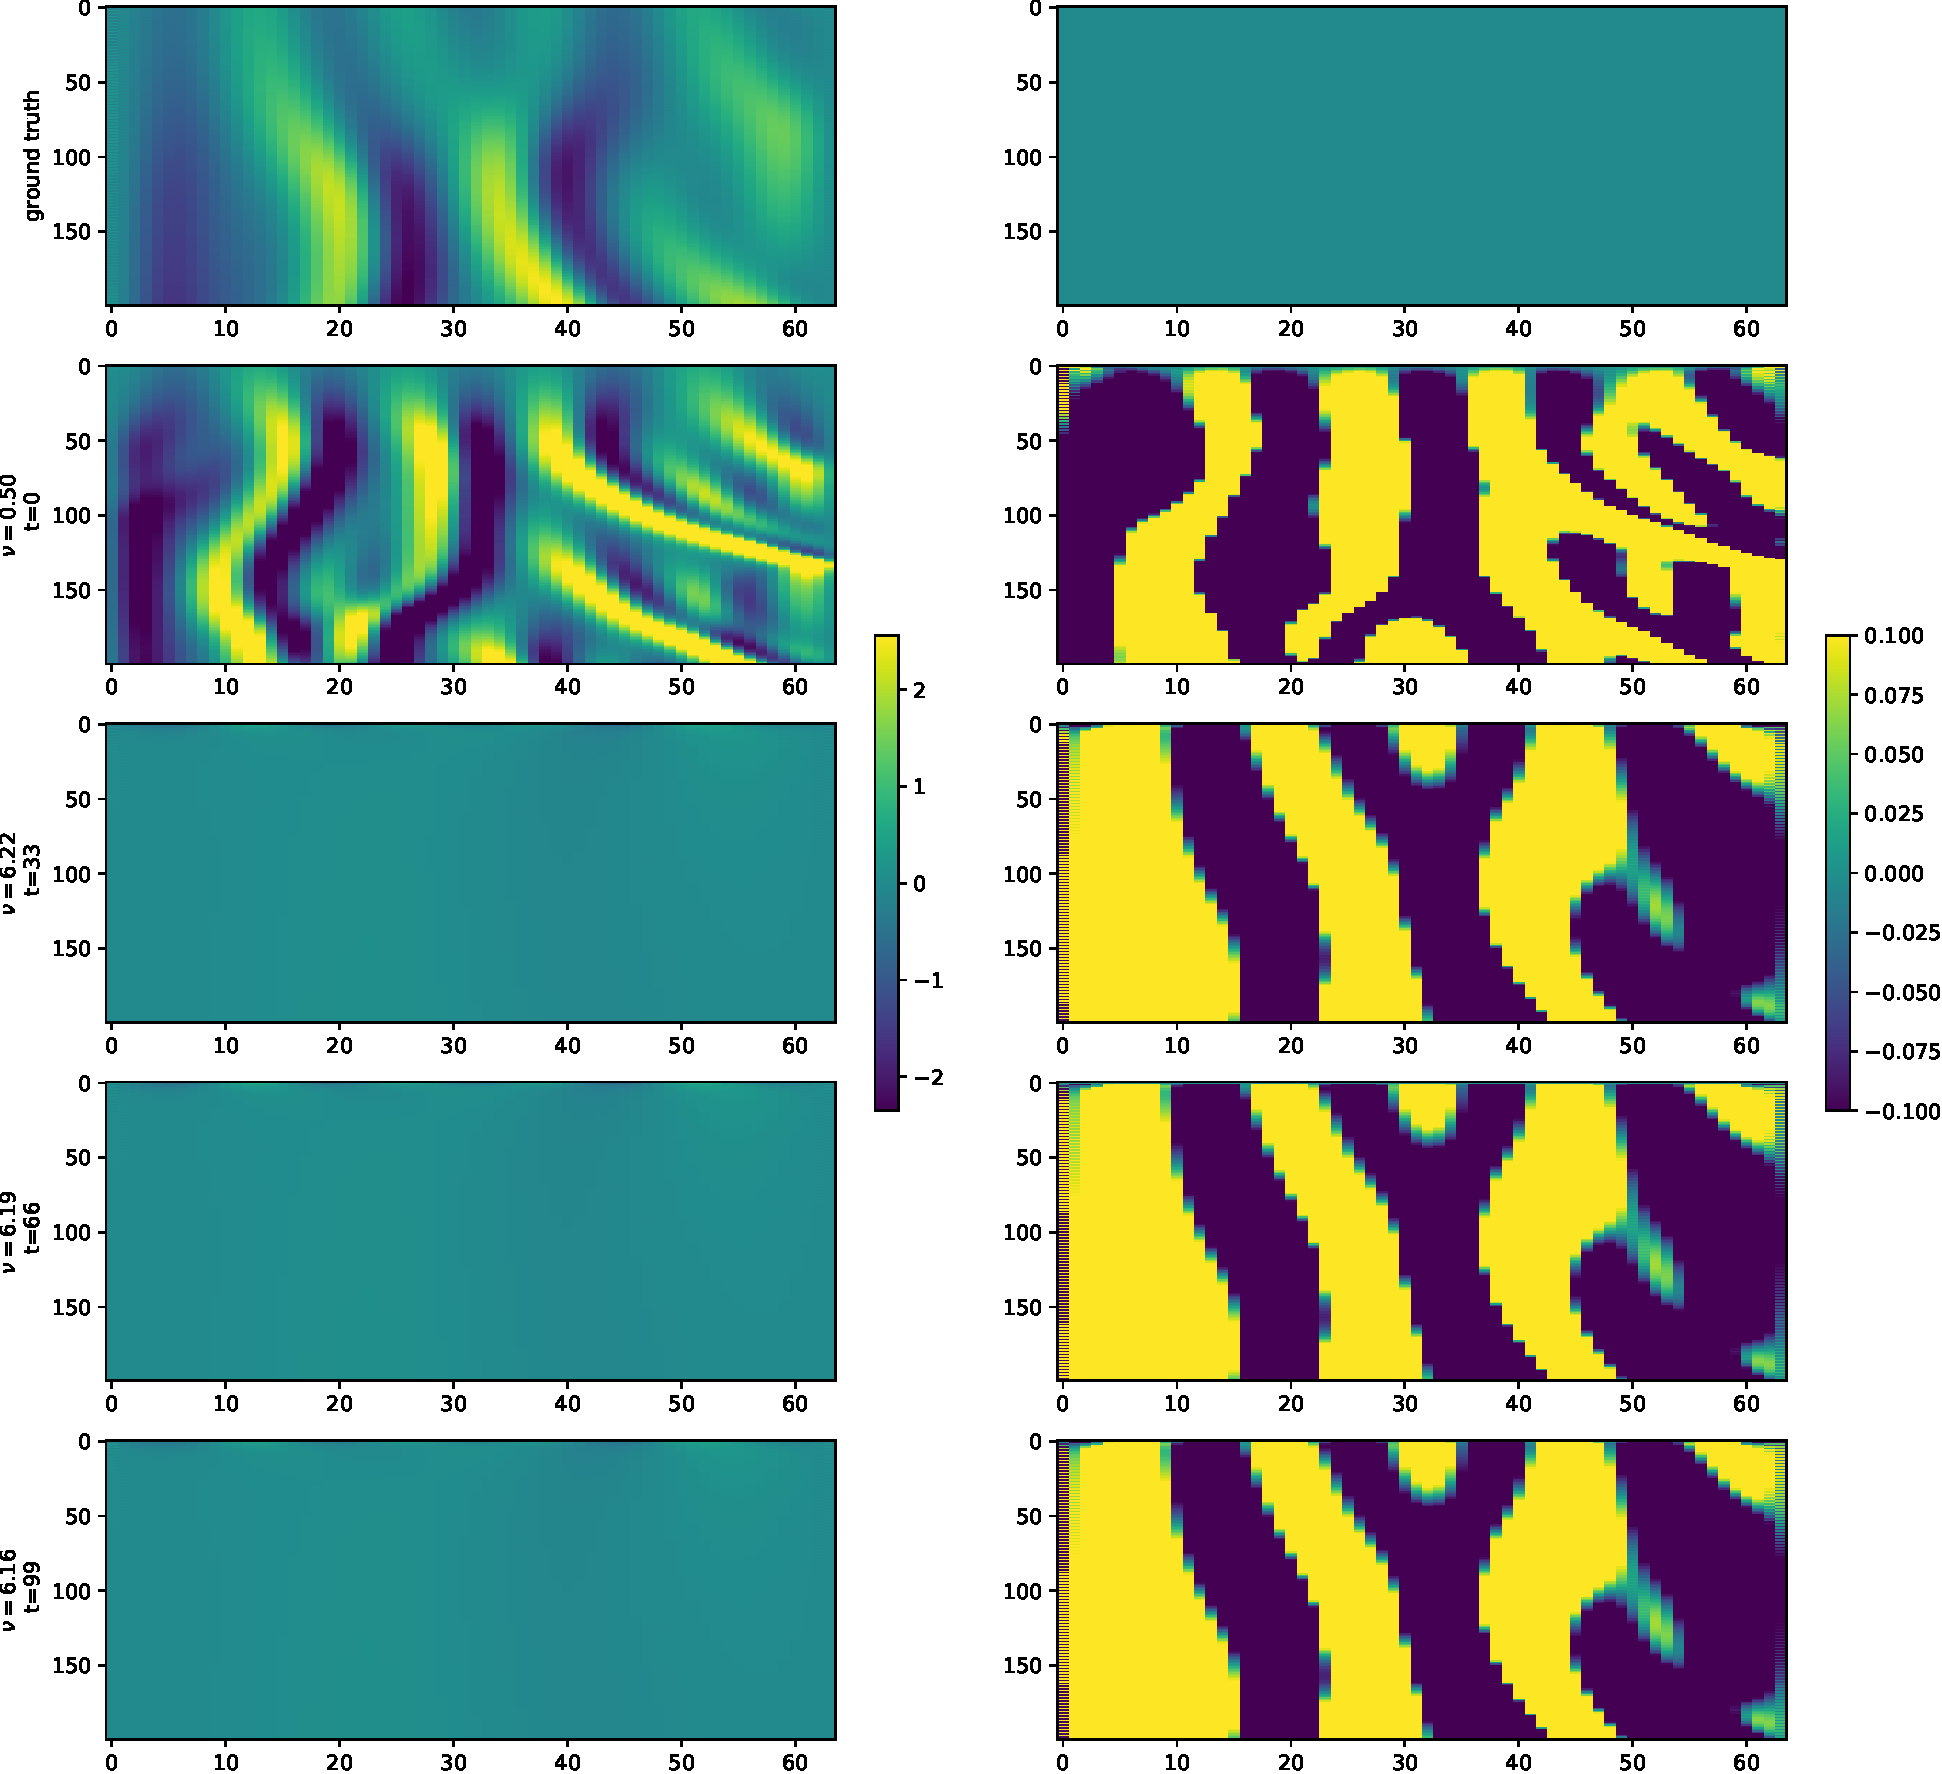
\includegraphics[width=\linewidth]{fig/ks-adjoint-cloudmap2.pdf}
			\caption{Adjoint method}
		  \end{subfigure}%
		  \begin{subfigure}{0.5\linewidth} % Adjust the width as needed
			\centering
			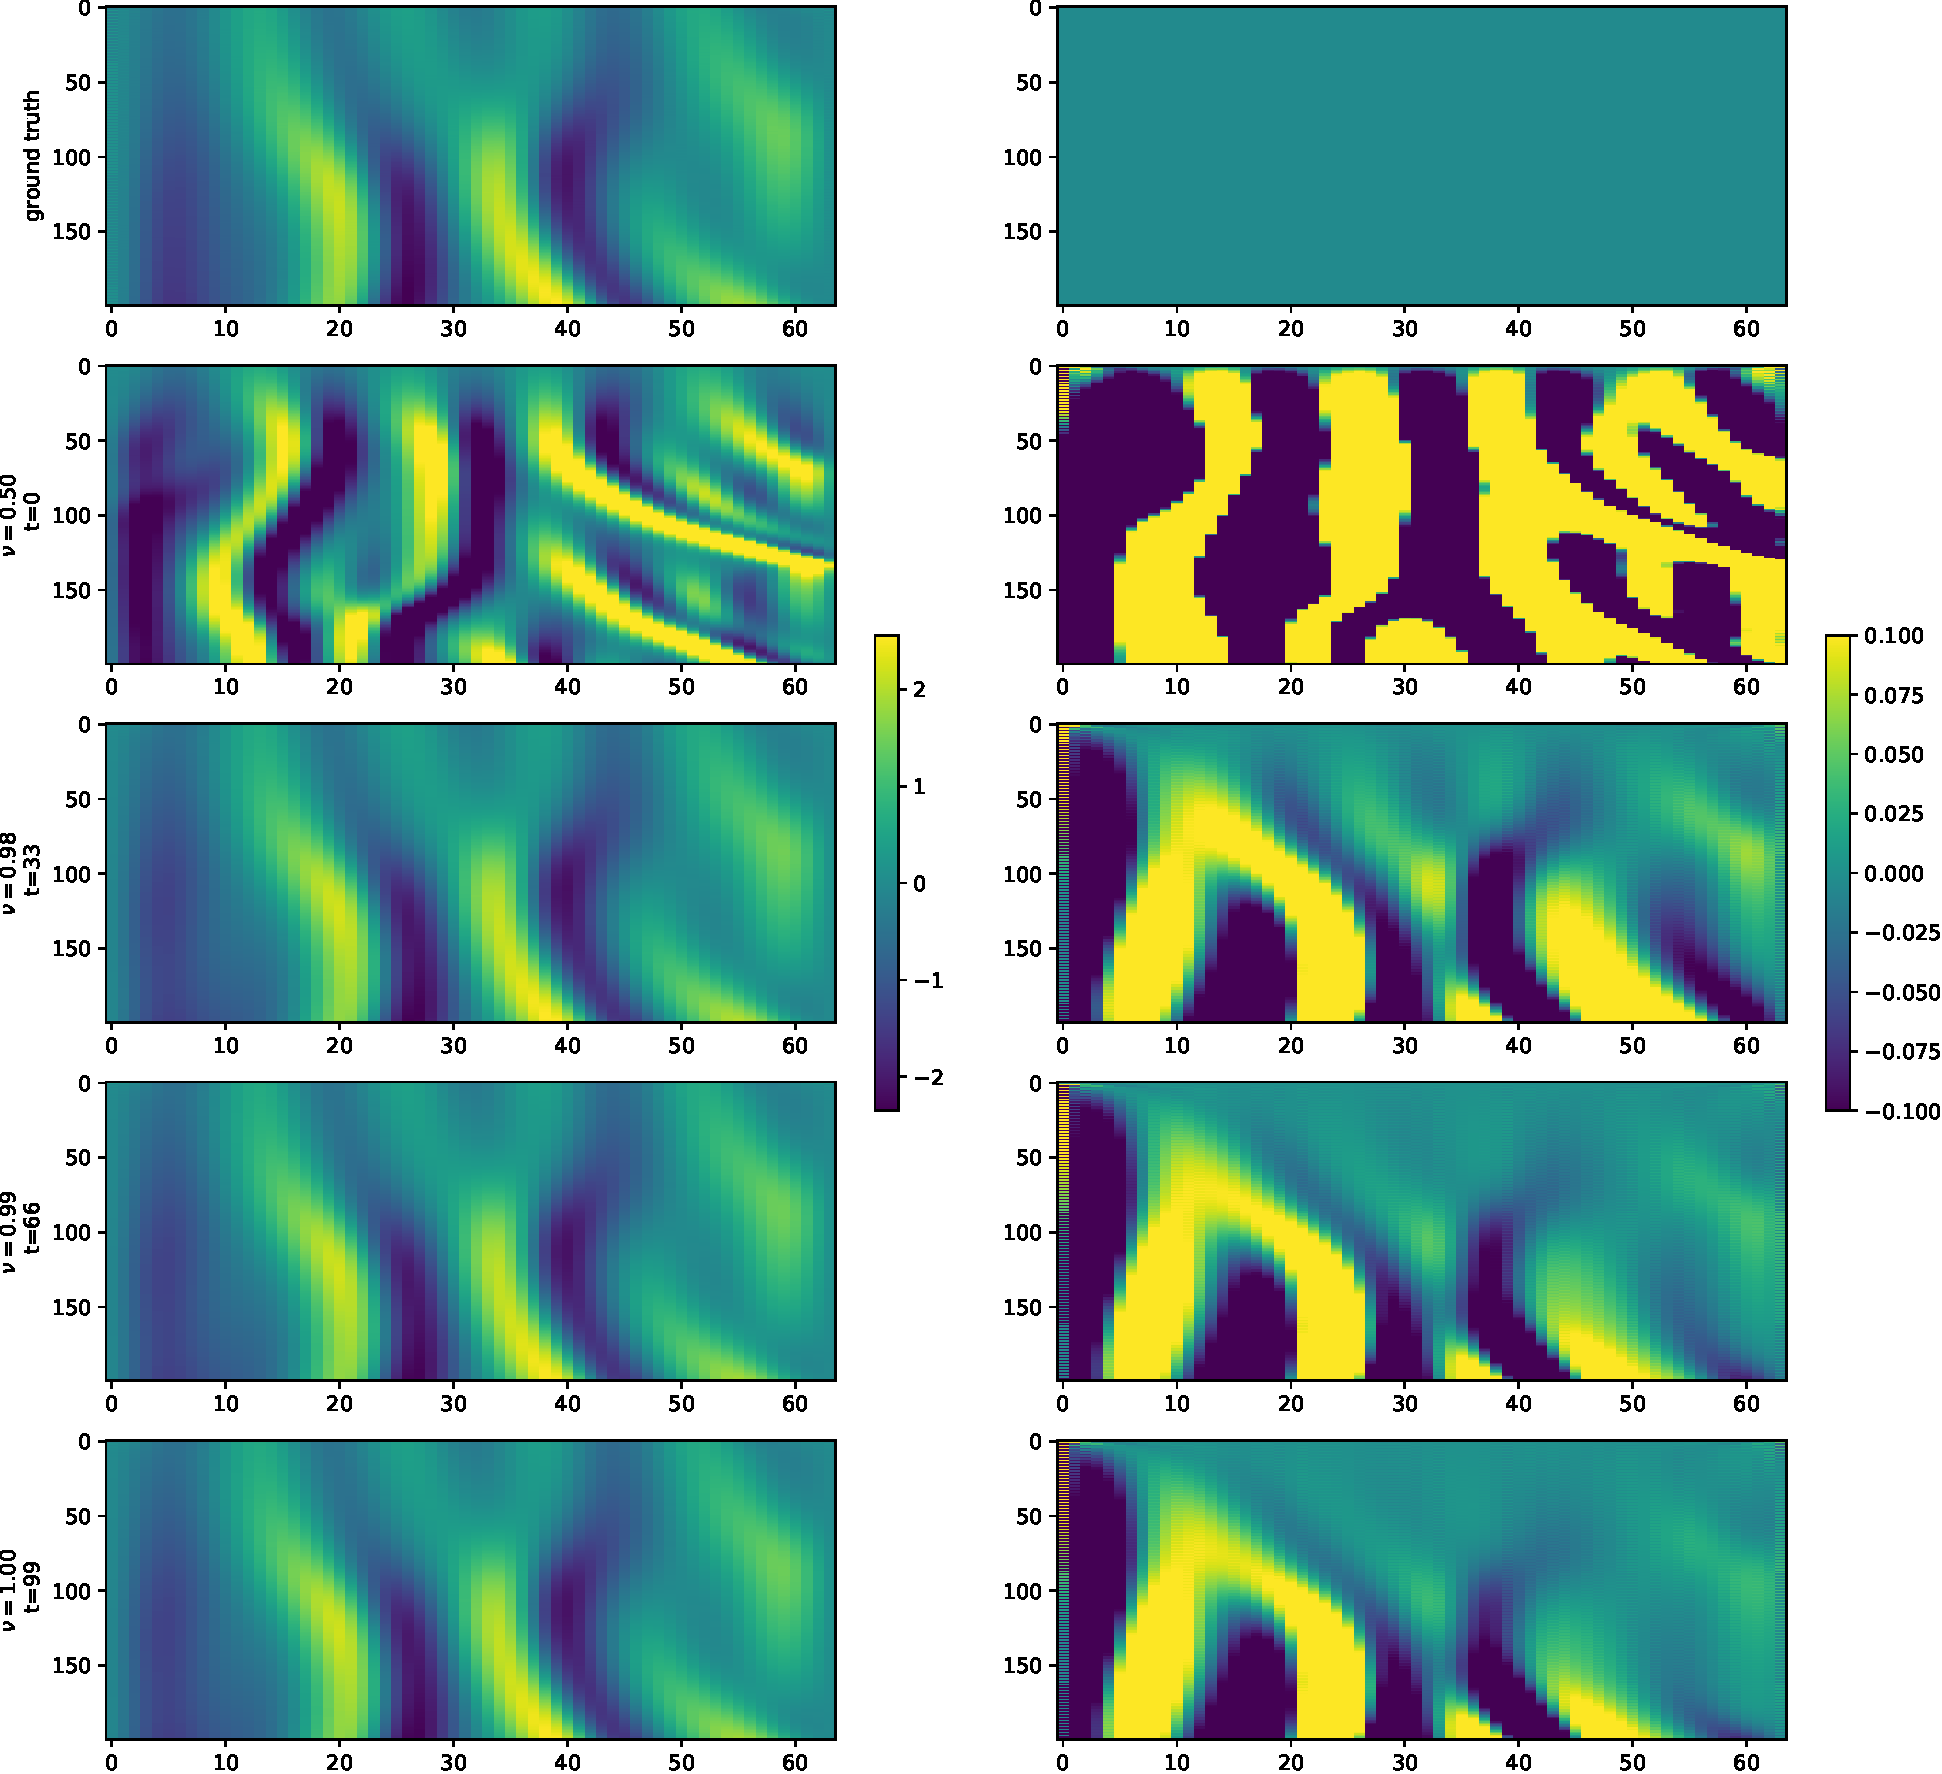
\includegraphics[width=\linewidth]{fig/ks-lss-cloudmap.pdf}
			\caption{LSS method}
		  \end{subfigure}
		  \caption{LSS for KS subgrid modeling}
\end{figure}
\end{frame}

\begin{frame}{Subgrid modeling of the 2D Navier-Stokes equation}
	Here, we consider a simple version of subgrid modeling for 2D NS equation:
	\bequ\label{NS}
	\p_t \mfu + (\mfu \cdot \nabla)\mfu + \nu\Delta \mfu = 0, \quad \nabla \cdot \mfu = 0,
	\eequ
	This corresponds to estimate the eddy-viscosity $\nu_t$ of LES subgrid modeling.
\end{frame}

\begin{frame}{Subgrid modeling of the Kuramoto–Sivashinsky equation}
	\begin{figure}[ht]
		\centering
		\begin{subfigure}{0.5\linewidth} % Adjust the width as needed
			\centering
			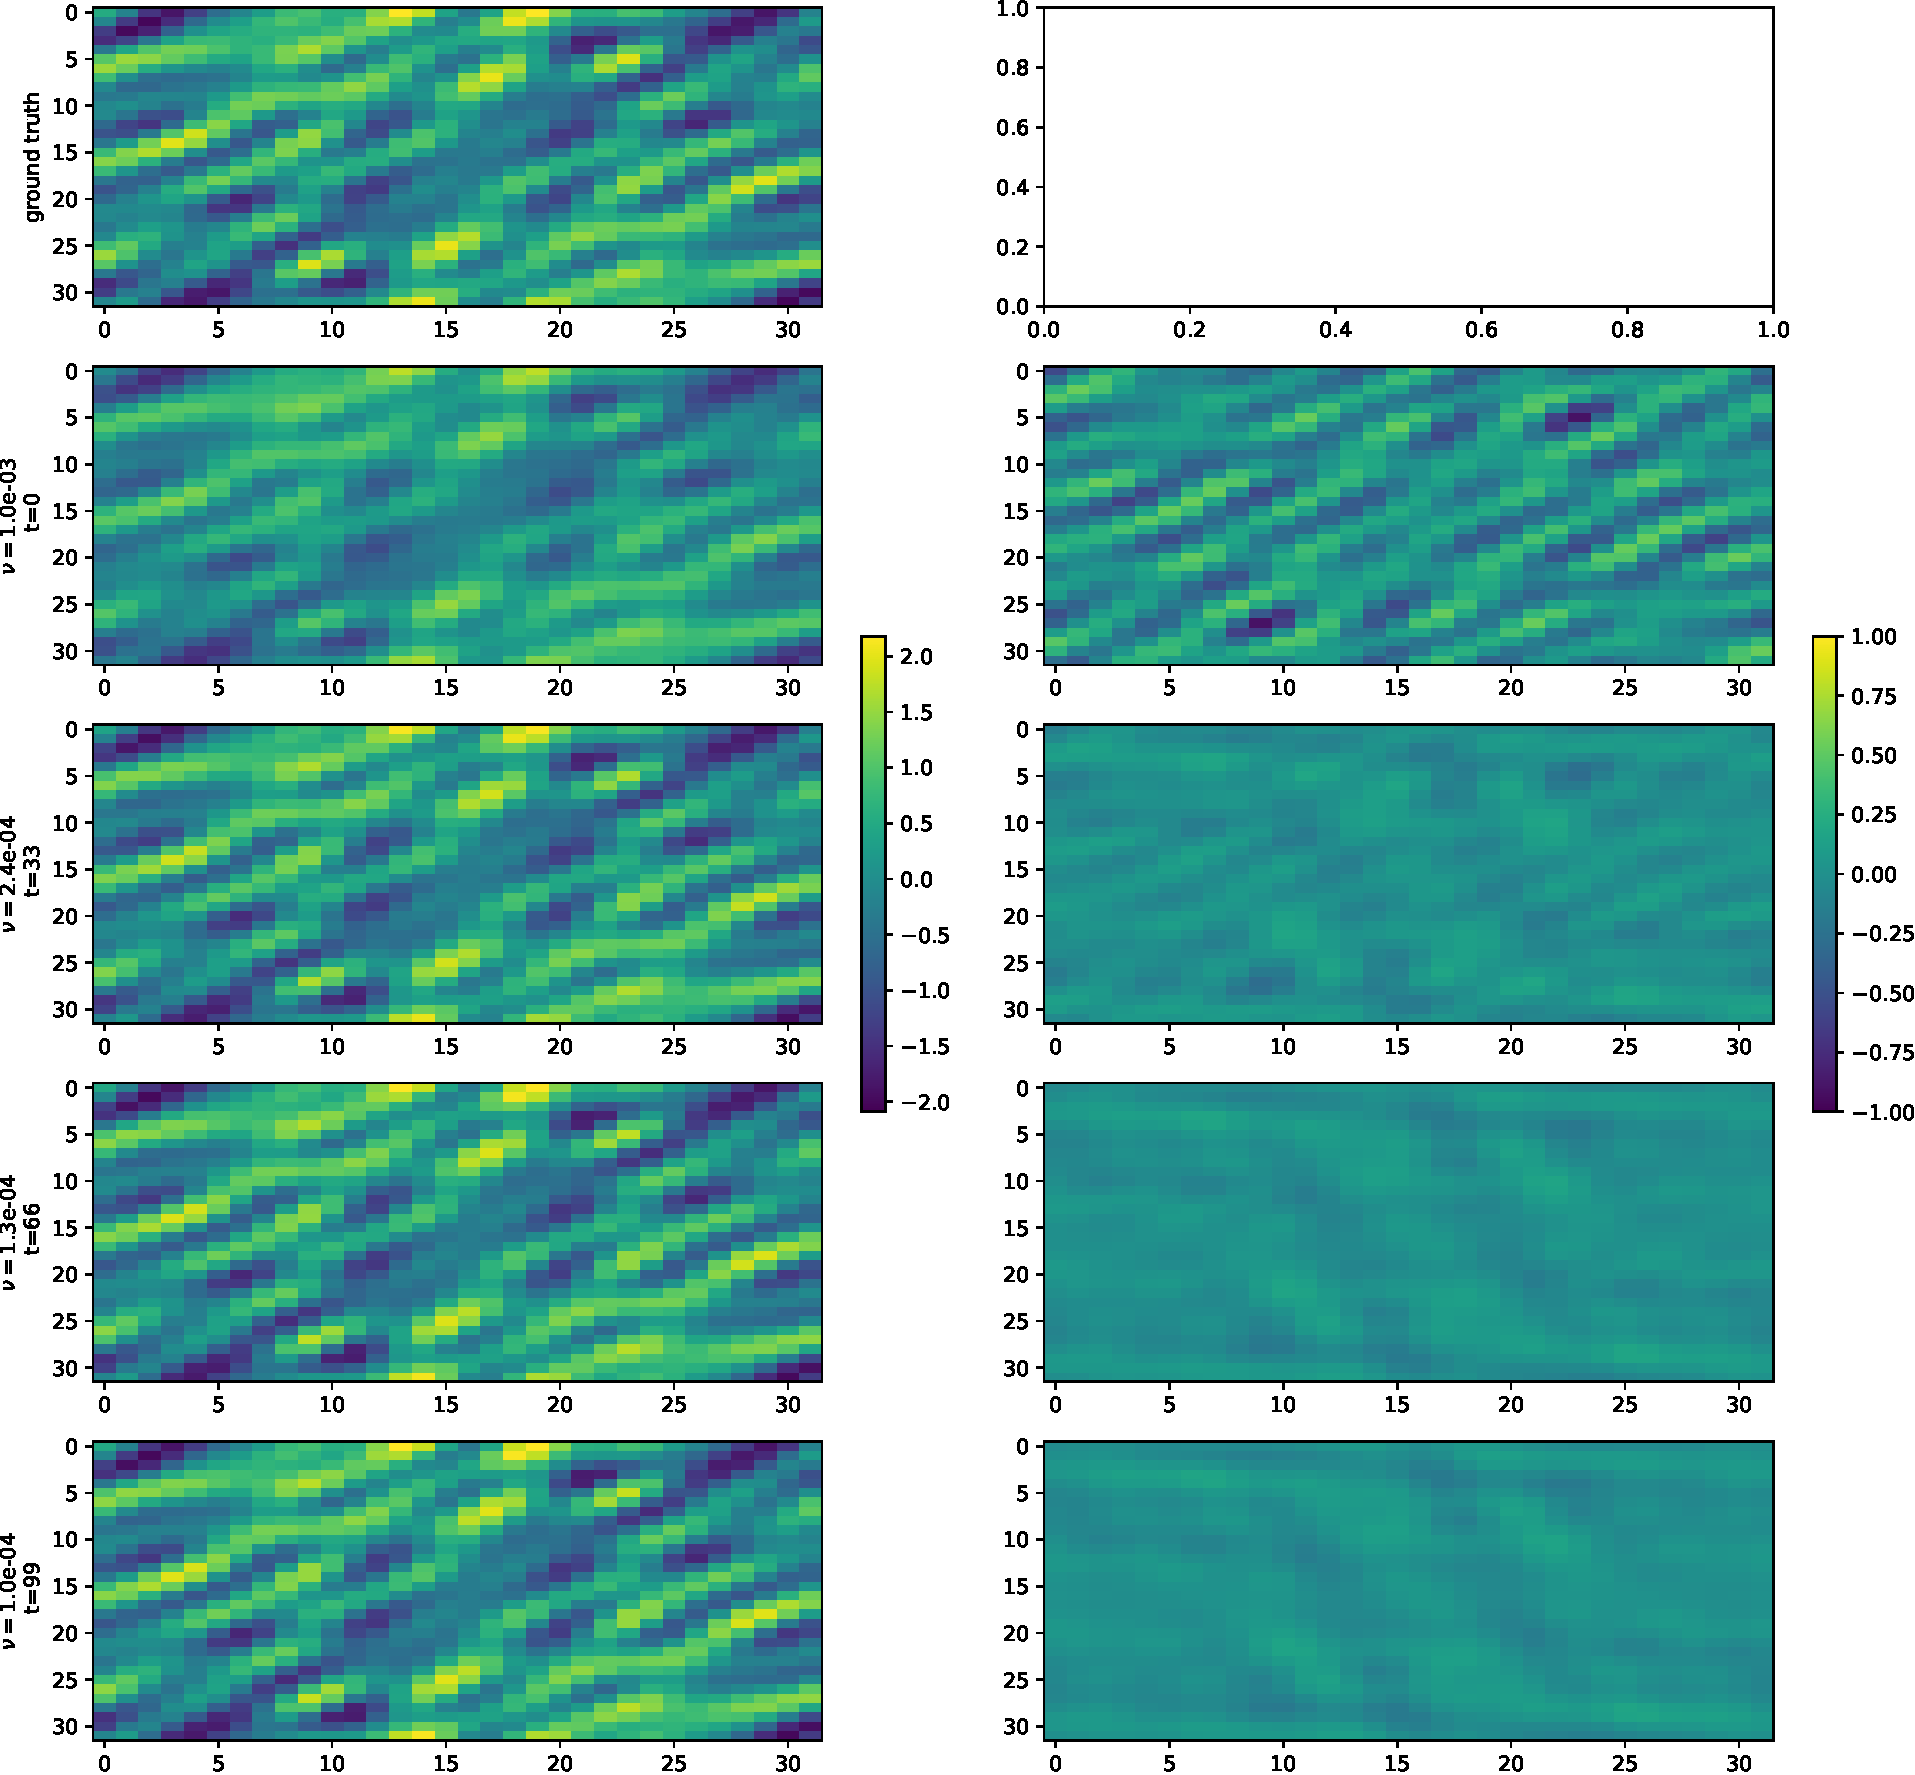
\includegraphics[width=\linewidth]{fig/ns-lss-cloudmap.pdf}
			\caption{Simulated configuration}
		  \end{subfigure}%
		  \begin{subfigure}{0.5\linewidth} % Adjust the width as needed
			\centering
			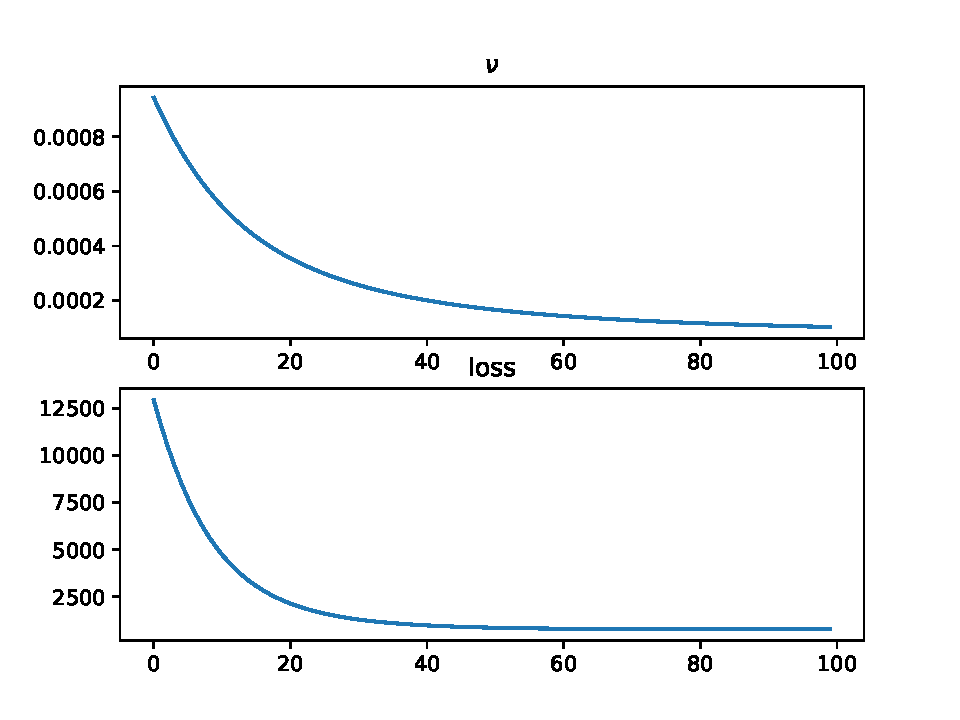
\includegraphics[width=\linewidth]{fig/ns-lss-nu.pdf}
			\caption{Error}
		  \end{subfigure}
		  \caption{LSS for NS subgrid modeling}
\end{figure}
\end{frame}

\begin{frame}{What is next?}
	\begin{itemize}
		\item[$\bullet$] Applying LSS (possibly via the help of neural network) to 2D isotropic turbulence to study the subgrid modeling and 
		sensitivity analysis of several model parameters. Moreover, implement scalable 
		method to work on the case of real world LES problem, e.g. 3D, more than 10M grid size, 
		and a reasonable long trajectory.
		\item[$\bullet$] Applying LSS to more complicated statistics which may also depends on the 
		initial contion (current method assume that the statistics is insensitive w.r.t. the
		inition condition).
		\item[$\bullet$] {\color{red}Viewing deep NN as a dynamics where layer depth is the time index, can we use 
		LSS to propose an algorithms to help calculating the gradient? Moreover, is there any other issue except
		for gradient vanishing and blow-up for deep NN?}
	\end{itemize}
\end{frame}

\begin{frame}{Reference}
	\begin{itemize}
		\item[$\bullet$] 1. C. Sparrow, The Lorenz Equations: Bifurcations, Chaos, and Strange Attractors, Springer-Verlag, New York, 1982.
		\item[$\bullet$] 2. Wang Q, Hui R, Blonigan P. Least squares shadowing sensitivity analysis of chaotic limit cycle oscillations. J Comput Phys 2014;267: 210–4.
	\end{itemize}

\end{frame}

\end{document}